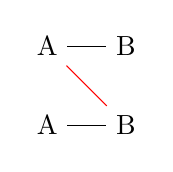
\begin{tikzpicture}
    \begin{scope}[name prefix = top-]
        \node (A) at (0,1) {A};
        \node (B) at (1,1) {B};
        \draw (A) -- (B);
    \end{scope}
    \begin{scope}[name prefix = bottom-]
        \node (A) at (0,0) {A};
        \node (B) at (1,0) {B};
        \draw (A) -- (B);
    \end{scope}

    \draw [red] (top-A) -- (bottom-B);
\end{tikzpicture}
